\title{Report for summer school CPS2018}
\author{
        \textsc{Lingyuan Yang}
            \qquad
        \\
        \normalsize
            \texttt{linyan@kth.se}
}
\date{\today}

\documentclass[12pt,twoside]{article}

\usepackage[paper=a4paper,dvips,top=1.5cm,left=1.5cm,right=1.5cm,
    foot=1cm,bottom=1.5cm]{geometry}


%\usepackage[T1]{fontenc}
%%\usepackage{pslatex}
\renewcommand{\rmdefault}{ptm} 
\usepackage{mathptmx}
\usepackage{amsmath}
\usepackage[scaled=.90]{helvet}
\usepackage{courier}
\usepackage{tikz}
\usetikzlibrary{arrows,decorations.pathmorphing,backgrounds,fit,positioning,calc,shapes}
\usepackage{pgfplots}
\pgfplotsset{compat=1.13}
\usepackage[center]{titlesec}
\usepackage{bookmark}

\usepackage{fancyhdr}
\pagestyle{fancy}

%%----------------------------------------------------------------------------
%%   pcap2tex stuff
%%----------------------------------------------------------------------------
 %\usepackage[dvipsnames*,svgnames]{xcolor} %% For extended colors


%% \usepackage{pgfmath}	% --math engine
%%----------------------------------------------------------------------------
%% \usepackage[latin1]{inputenc}
\usepackage[utf8]{inputenc} % inputenc allows the user to input accented characters directly from the keyboard
\usepackage[english]{babel}
%% \usepackage{rotating}		 %% For text rotating
\usepackage{array}			 %% For table wrapping
\usepackage{graphicx}	                 %% Support for images
\usepackage{float}			 %% Suppor for more flexible floating box positioning
\usepackage{color}                       %% Support for colour 
\usepackage{mdwlist}
%% \usepackage{setspace}                 %% For fine-grained control over line spacing
%% \usepackage{listings}		 %% For source code listing
%% \usepackage{bytefield}                %% For packet drawings
\usepackage{tabularx}		         %% For simple table stretching
%%\usepackage{multirow}	                 %% Support for multirow colums in tables
\usepackage{dcolumn}	                 %% Support for decimal point alignment in tables
\usepackage{url}	                 %% Support for breaking URLs
\usepackage[perpage,para,symbol]{footmisc} %% use symbols to ``number'' footnotes and reset which symbol is used first on each page

%% \usepackage{pygmentize}           %% required to use minted -- see python-pygments - Pygments is a Syntax Highlighting Package written in Python
%% \usepackage{minted}		     %% For source code highlighting

 \usepackage{hyperref}		
\usepackage[all]{hypcap}	 %% Prevents an issue related to hyperref and caption linking
%% setup hyperref to use the darkblue color on links
 \hypersetup{colorlinks,breaklinks,
             linkcolor=darkblue,urlcolor=darkblue,
             anchorcolor=darkblue,citecolor=darkblue}

%% Some definitions of used colors
\definecolor{darkblue}{rgb}{0.0,0.0,0.3} %% define a color called darkblue
\definecolor{darkred}{rgb}{0.4,0.0,0.0}
\definecolor{red}{rgb}{0.7,0.0,0.0}
\definecolor{lightgrey}{rgb}{0.8,0.8,0.8} 
\definecolor{grey}{rgb}{0.6,0.6,0.6}
\definecolor{darkgrey}{rgb}{0.4,0.4,0.4}
%% Reduce hyphenation as much as possible
\hyphenpenalty=15000 
\tolerance=1000

%% useful redefinitions to use with tables
\newcommand{\rr}{\raggedright} %% raggedright command redefinition
\newcommand{\rl}{\raggedleft} %% raggedleft command redefinition
\newcommand{\tn}{\tabularnewline} %% tabularnewline command redefinition

%% definition of new command for bytefield package
\newcommand{\colorbitbox}[3]{%
	\rlap{\bitbox{#2}{\color{#1}\rule{\width}{\height}}}%
	\bitbox{#2}{#3}}

%% command to ease switching to red color text
\newcommand{\red}{\color{red}}
%%redefinition of paragraph command to insert a breakline after it
\makeatletter
\renewcommand\paragraph{\@startsection{paragraph}{4}{\z@}%
  {-3.25ex\@plus -1ex \@minus -.2ex}%
  {1.5ex \@plus .2ex}%
  {\normalfont\normalsize\bfseries}}
\makeatother

%%redefinition of subparagraph command to insert a breakline after it
\makeatletter
\renewcommand\subparagraph{\@startsection{subparagraph}{5}{\z@}%
  {-3.25ex\@plus -1ex \@minus -.2ex}%
  {1.5ex \@plus .2ex}%
  {\normalfont\normalsize\bfseries}}
\makeatother

\setcounter{tocdepth}{3}	%% 3 depth levels in TOC
\setcounter{secnumdepth}{5}
%%%%%%%%%%%%%%%%%%%%%%%%%%%%%%%%%%%%%%%%%%%%%%%%%%%%%%%%%%%%%%%%%%%%
%% End of preamble
%%%%%%%%%%%%%%%%%%%%%%%%%%%%%%%%%%%%%%%%%%%%%%%%%%%%%%%%%%%%%%%%%%%%

\renewcommand{\headrulewidth}{0pt}
\lhead{CPS2018}
%% or \lhead{II2202, Fall 2016, Period 1}
\chead{Final project report}
\rhead{\date{\today}}

\makeatletter
\let\ps@plain\ps@fancy 
\makeatother

\setlength{\headheight}{15pt}
\begin{document}

\maketitle

\centering
\section*{Executive summary}

This report is for the cyber security and privacy summer school 2018 in Trento. The name of our project
is EspioNo. We provide device to secure your private conversation from listening by smart speakers.
With a state-of-art technology disturbs the microphone but not human ear.
To introduce our project, this report is divided into 4 sections.
The first section will be focusing on the process of idea generation and optimization, as well as the technical basement.
The second section will be introducing our business canvas, detailize our business structure.
The third section will introduce our time line and expected cash flow. And the last section will evaluate the performance 
of myself both as a participant of summer school and a member of a team.



\clearpage

\selectlanguage{english}
\tableofcontents



\clearpage
\rr

\section{Problem and solution}
\label{sec:Problem and solution}
\subsection{Problem addressment}
From the point that Amazon post its 90 seconds 'Alexa Loses Her Voice' advertisment, people begin to fascinate with smart speakers 
for the convenience it introduce into our life. However, to interacte with the users, smart speaker has to keep listening to them. 
This feature arise doubt and panic on privacy issue. Some reports publised recently seems to confirm that such concern make sense. 
According to The New York Times \cite{nyctimesalexa} and Quartz \cite{quartzalexa}, alexa sometimes do record undesired conversation and 
even send it to other people. If this happens, why can't they tap us and make money by our privacy? Such tapping problem is a big worry 
for people who care about privacy. And the patent of Google and Amazon It's also been heard that when people talk about something they 
like or they want, an relative advertisment will be forwarded to them soon.
A study has been done across America showing that 54\% of the adults of the United States do not own a smart device in their home. 
6.4 milion people said specifically they would not buy a smart speaker due to privacy reasons. 6.4 million people. And what about 
the 20 million people who want to increase their privacy. In the united states alone, we have not even talked about the rest of the world. 
And this problem will only increase in the future. \\
In this case, the problem we are going to solve is that people want to keep privacy while using smart speaker without undermine the convenience.


\subsection{Problem validation}
We use two ways to validate our problem. The first one is talking with people. The second way is reading reports and statistics about 
such problem. Firstly, we talk to people who has a smart speaker, 4 of our relatives are involved into our interview and all of them 
confirm that they do have such concern and they are willing to pay for products solving such trouble. We also happen to have  
"interivews" with Mr Jovan senior and junior during technical consulation and montoring slot. They both think Amazon and Google are 
not trustworthy and would like to have solutions for such problem, they represent the group of people who show interest about smart 
speaker but don't buy them due to privacy concerns.\\
We also collect statistics to validate our problem. According to a research conducted by Pew Research Center, 46\% of the American adults 
have ever use digital voice assistants while 8\% say they have ever use a stand-alone device such as Amazon Echo or Google Home. 
In the mean while, according to a survey from Business Insider \cite{privacyfear} 40\% of people are concerned about connected-home 
devices tracking their usage. And according to Business Wire , 6.4 million people said specifically they would not buy a smart 
speaker due to privacy reasons.

\subsection{Solution and validation}
\subsection{Proposed solutions}
To solve the addressed problem, we brainstorm and come up with several solutions and validate them one by one.
Generally speaking, there are three ways preventing smart speaker from tapping.
\begin{itemize}
\item \textbf{Cut off power supply when not used } This way is to make a smart switch with speech recognition function to shut down the 
smart speaker when you don't want to use it anymore.
\item \textbf{Monitor/Control the internet connection when not used} This way is to stand in between remote server and local speaker 
monitor all the internt traffic to secure no sensitive data been transmitted.
\item \textbf{Physically prevent smart assistants from listening} This way is to disturb or deafen the microphone on smart speaker, 
make them unable to heard from us. And remove the interference when desired.
\end{itemize}

\subsection{Validation process}
In the beginning, these three solution all looks hopeful. But two of them are deprecated after we reading technical literature and doing test.
\begin{itemize}
\item \textbf{Why we abandon power switch solution} This solution is easy to validate. There is no doubt that it will work. But the problem is 
how well it works and if it's convenient. We do have a google home to conduct experiment. After we turn it off and reboot, it takes about 
1 minute to be responsive again. Which means if we are going to use such solution, every time our customer want to use smart assistant they 
will have to wait for 1 minute after they say the key word.\\
Customer buy smart speaker for the convenience. If our product makes life harder, it does't make sense and nobody will pay for it.
In this case, we kill this solution first, even before look into technical detail.
\item \textbf{Internet monitor solution} This solution actually include two different solution, internet switch and 
package sniffing. The second one is the inproved version of first one.\\
The internet switch is what we originally come up with during brain storm. It works just like power switch, but instead of control over power, 
it controls upload traffic, prevent package being transmitted when not desired. The best thing about this solution is that it eliminates the 
drawback of booting latency. However, as long as we don't know the mechanism behind, we cannot ensure that the tapped audio won't be transmitted 
once reconnected to the internet. \\
With such problem, we consult Yvo Desmedt during a consulation slot we booked. He suggest us to use sniffing technology to monitor what is
actually transmitted. In other words, our product will act as a transfer center of package from smart speaker and analize the package to 
figure out if undesired package is being transmitted.
With this suggestion, we do research and find out the audio data being transmitted are encrypted \cite{googlepolicy}, which make sniffing 
work extremly hard. And it turns out somebody has already do simmilar job and we can derectly refer to it. According to a report 
\cite{sniffingresult} by Maik Morgensternfrom AV-TEST, the communication channel of Amazon Alexa uses TLS1.2 encryption with certificate 
validation/pinning. This technique prevented them to use a Man-In-The-Middle-proxy and read along the encrypted traffic. So they creat a 
scenario to evaluate the intensity of data transimission and estimate what is being transmitted. The scenario strats with 8 seconds of silence 
and then Asking Alexa “What time is it?” (~6 seconds), then another 8 seconds of silence and followed by “Alexa – tea, earl grey, hot” and 
await the answer (~5 seconds) finally the scenario end with 23 seconds of a normal conversation between two people (not including any Alexa keywords).
 
\begin{figure}[!htb]
\centering
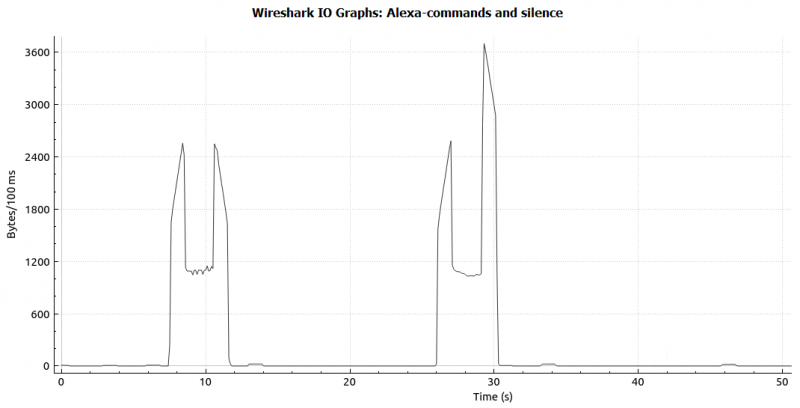
\includegraphics[width=0.6\textwidth]{alexa_wakeup_and_pause-400x204.png}
\caption{Transmitted bytes in the given scenario}
\label{fig:Transmitted bytes in the given scenario}
\end{figure}

We can see the result from figure \ref{fig:Transmitted bytes in the given scenario} that the data transimission during conversation looks simmilar with
silent time, it is very likely that Alexa do not send data if it's not working. This analisis is unfavorable to our solution.\\
Also, Prof. Yvo Desmedt give us an artical \cite{bourse2017fast} about homomorphic encryption. With such technology we will be able to processing data, 
such as speech recognition, on remote server encryptedly wothout let the server konw a peice of information. To make use of such advanced technology 
we need to build our own smart speaker and the remote server to conduct homomorphic encrypted speech recognition. These is not viable for starting point, 
we plan to include it in our long term plan. 

\item \textbf{Audio disturbing solution} Interference is the first solution we come up with. The way how it works is to decrease the Signal Noise Ratio(SNR), 
which describe the level of a desired signal to the level of background noise, as low as possible. In other word, make noises to make conversation 
incomprehensive. There is one thing to be noted, a startup company called Privacy Shield has already 
\begin{itemize}
\item  The first version of disturbing solution: use mini speakers to play white noise, which is a very common noise type, near the 
microphone of smart speaker. However, there is a big problem. The noise we play might bother our customer. According to the Acoustic Modeling report
of google home \cite{46130}, it could work well at SNRs ranging from 0 dB to 20 dB or above. So in the most optimistic scenario, we need to decrease the SNR 
to 0 dB which means the noise is as loud as human voice when reaching the microphone. This is load enough to be haerd several meters away.
\item The second version of our solution: use a case to cover the smart speaker which could both decrease the volume of human voice reaching microphone and 
the volume of noise needed. A case could fix the problem in the first version almost perfectly, it both decrease the volume of noise we need and the volem of 
noise leak out. But we need a mechanical structure to open and close the case, which should also be audio-controled. The way it work is shown in 
figure \ref{fig:Audio disturbing solution}. This structure is viable although it require complicated mechanical structure to support smooth opening and 
closing of the case and also speech recognition function to remain the user experience. Not good enough but we still use this solution for our first pitch.
\begin{figure}[!htb]
\centering
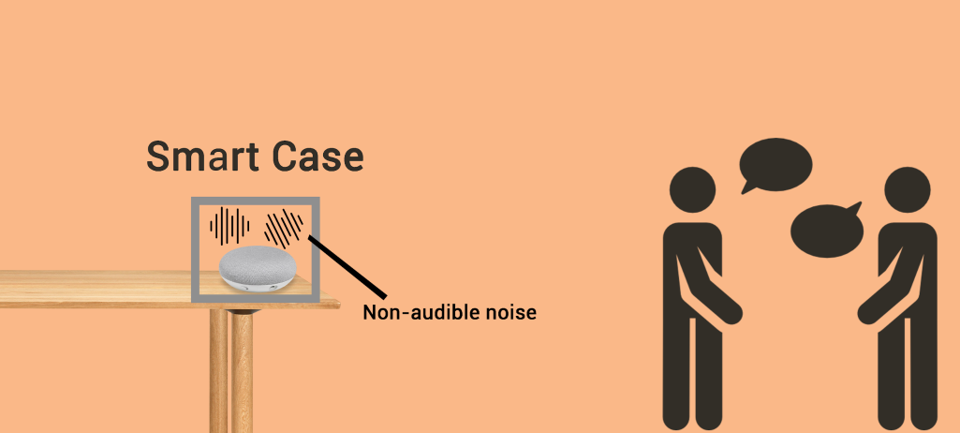
\includegraphics[width=0.6\textwidth]{case.png}
\caption{Audio disturbing solution}
\label{fig:Audio disturbing solution}
\end{figure}
\end{itemize}

\end{itemize}

\subsection{Final solution}
The final solution actually evolved from the second version of Audio disturbing solution. After struggling on simplify our product and trying to add encryption 
elements to the solution. Fortunately, we found a newly published artical from UIUC \cite{RoyNirupam2017BMMH} which provide a way to use inaudible ultrasonic sound
to disturb microphones.\\

\begin{figure}[!htb]
\centering
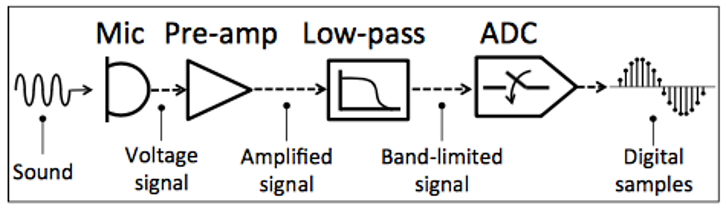
\includegraphics[width=0.6\textwidth]{mic_circuit.png}
\caption{Circuit inside microphone}
\label{fig:Circuit inside microphone}
\end{figure}
Inside the microphone, all the physical audio will first been transfered to electronic signal, after that the signal should pass a component called pre-amplifier 
which will amplify the analog signal to make sure it can be effectively measured by ADC. In this procedure, the output of pre-amplifier is linear only when input 
is in the audible frequency range which is 10-23 KHz, outside this range, the response exhibits non-linearity which will introduce harmonic. In the artical, 
by making use of such non-linearity, they design the input ultrasonic sound and make a controlable shadow noise signal within the audible range, which has been
perfectly recorded by microphone.

\begin{figure}[!htb]
\centering
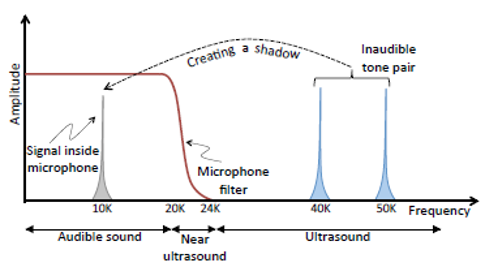
\includegraphics[width=0.6\textwidth]{shadow.png}
\caption{Use ultrasound to generate shadow noise}
\label{fig:Use ultrasound to generate shadow noise}
\end{figure}

And by analyze the output signal from pre-amplifier, the researchers make sure that the "shadow" noise is as expect and strong enough to disturb the speech 
recognition result. Being more specific, they use two tones at say 40kHz and 50kHz, When these tones arrive together at the microphone's power amplier,
they are amplied as expected, but also multiplied due to fundamental non-linearities in the system. Multiplication of frequencies f1 and f2 result in frequency 
components at $(f_1-f2)$ and $(f_1+f_2)$,  $(f_1-f2)$ is 10kHz in this case. The harmonic measured is shown in figure \ref{fig:Non-linear Harmonic}.

\begin{figure}[!htb]
\centering
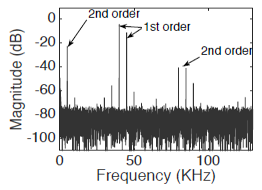
\includegraphics[width=0.5\textwidth]{freq.png}
\caption{Non-linear Harmonic}
\label{fig:Non-linear Harmonic}
\end{figure}

This solution is perfect for the problem we addressed, however, we still facing questions during technical consulation.

\begin{itemize}
\item \textbf{Will the ultrasound hurt people?}\\ The first obvious concern is about health and well-being, people are always worry about radiation and altrasound 
hurt their health. Actually ultrasound effect your body just as normal sound, frequency here does not make any difference. Only power of the voice matters 
\cite{ultrasoundfda}. According to the measurement conducted by the auther\cite{RoyNirupam2017BMMH}, we know that the amplifier have a very large magnitude, which is 
-40 dB/Hz around frequency of 45kHz, this means we can make our disturbing altralsound really weak to fulfill the desired effect.
\item \textbf{Will the ultrasound hurt pets?}\\ We know that the audible range of pets like dogs and cats are different from people, usually higher. What if the 
frequency of ultrasound is out of human audible range but fall in animal hearing range? This concern make sense. We have choice to design the frequencies of input 
ultrasound as long as their difference remian the same, however, the further the frequency deviates from 50kHz, which is a peak for magnitude, the smaller the 
amplification. This problem can be solved, although not perfectly right now.
\item \textbf{This technology is brand new, is it business viable?}\\ Our solution s based on a paper published last year. Such new technology could help us get rid 
of much competition, but also rise the problem that if it can be realize. According to the paper the authers already have a prototype for testing, and by reviewing 
the blog of the authers, we found out the prototype they made \ref{fig:Prototype}. It's a speaker array to disturb the microphone in a room, while the power of it is 
only 2W. \\
We also write email to cantact with them. Their technology is pending for IP but they welcome usage for research and also open for business coorperation.

\begin{figure}[!htb]
\centering
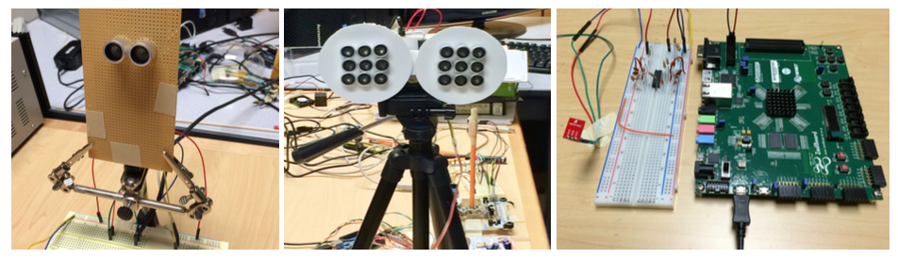
\includegraphics[width=\textwidth]{prototype.png}
\caption{Prototype}
\label{fig:Prototype}
\end{figure}

\end{itemize}

After all of these problem we finalize the desining of our product. Which is shown in figure \ref{fig:Final designing}

\begin{figure}[!htb]
\centering
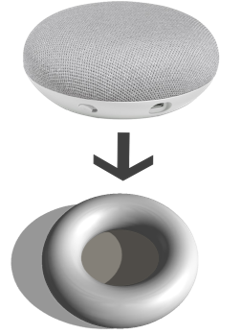
\includegraphics[height=0.6\textwidth]{safedock.png}
\caption{Final designing}
\label{fig:Final designing}
\end{figure}






\section{Business modelling and planning}
\label{sec:Business modelling and planning}
In our case, business modle is relative straightforward. We develope product and sell them. Which is called directly sale modle.
\subsection{Business modelling}
\begin{itemize}
\item \textbf{Key Partners}\\
    \begin{itemize}
    \item \textbf{The authers of article} \cite{RoyNirupam2017BMMH}. As long as the technology we rely on is based on others IP, or very likely 
    have an IP. We need to coorperte with them. Not only for technical development support, but also to prevent infringement of 
    intellectual property rights.
    \item \textbf{Google \& Amazon} Our business is dependent on the development of smart speaker. Right now, Google Home and Amazon Alexa combining 
    account for 90\% of market share. They are special to our business, our product are against them while we also dependent on their progress.
    These giants won't stand by and watch us standing in their way, they will have some way to solve this problem. Instead of waiting for competition with 
    these giants, which would be tough for our start-up, we have choice to get in touch with them and seek some kind of coorperation or even been bought 
    in the future.
    \item \textbf{Speech recognition special company} One of the key value of our product is that we do not hurt the convenience. As long as we need a 
    speech recognition solution which ought to work as better as Google does, it is wise to find a partener who is specialized in this area. 

    \end{itemize}

\item \textbf{Value Proposition}\\
\begin{itemize}
    \item \textbf{Keep privacy for our customer} The core value of our product is keeping privacy, to prevent Google and Amazon from tapping ourcustomer
    and also to make our customer feel secured.
    \item \textbf{Remain convenience} The most important reason for using a smart sepaker is to make life easier, our product should be a gain for smart speaker 
    in which case we will keep the feature of audio control and fast response.
\end{itemize}

\item \textbf{Customer Segments}\\
\begin{itemize}
    \item \textbf{People who already have a smart speaker.} This group of people is the so called early adopters who are willing to try fresh things. They are very 
    likely having such trouble. Acoording to the survey \cite{amountsmartassistant}, 40\% of the users of smart speaker do worry about privacy issues. And our 
    product perfectly fit their demands. They are also proven customers who have willing to pay for such advanced products.
    \item \textbf{People who want a smart speaker but do not for privacy reason} The number of this group of people is considerable, while the willing to pay is 
    hard to say. With the survey \cite{privacyfear} conducted by Business Insider we can say that we have 6.4 million potential customer in this group. The problem 
    here is how to strengthen their will to pay.
\end{itemize}

\item \textbf{Channels}\\
In the beginning, we will only focus on the online channel. After we start to profit, we will start to touch with physical retailor and promote our product.
\begin{itemize}
    \item \textbf{Online direct sale} From the financial lecture given by Vittorino, we know that sale through retailor will dramatically increase the cost, which 
    including profit sharing, charges for putting on shelf and transportation etc. Which make it hard to make profit in the beginning. So our plan is to build up our 
    own website first, and open for pre-oder, which help us estimate the interest of potential customers, have provment to ask for investment and increase the profit 
    margin.
    \item \textbf{Retailor} For long term plan, physical store is necessary. We need chance to display the functionality in real to convince people rather than barely
    show the demo video. And, also we need physical nodes to support maintenance job. Physical retailor will be a great solution to such problem. However, this 
    distribution channel would ONLY be a supplement for online direct sale. This is not only because of the high costs, but also because most of smart speakers are sold
    online, like google home through google store and Alexa through Amazon. Online shopping is one of the tendency of our potnetial customer. 
\end{itemize}

\item \textbf{Competitors}\\
\begin{itemize}
    \item \textbf{Privacy Shield} This is a start-up called \href{https://getprivacyshield.co/}{Privacy Shield}. The only start-up who are working on the same problem.
    Their product is aiming on Amazon Alexa, the most popular smart speaker right now. It is a cover on top of Alexa, generating noise to disturb microphone. From the 
    demo video we can see that their product is kind of bulky. With that cover, Alexa alomost became a colum. And according to the description, this device need to be 
    turn on and off physically by hand, which decrease the usibility and convenience. Even though they are one step ahead of us, their product is not specifically match 
    the market position of us.
    \item \textbf{Do it yourself} Although can not be count as a product or competiter, this is a very common way for people to solve such problem. People like my parents
    do not trust such device, they will turn off the speaker when they are not using them. Some people also use tap to seal the microphone, although it doesn't work well.
    This kind of solution is extremly cheap or even free. But it has the worst user experience.
    \item \textbf{Google \& Amazon} As the manufacturer of smart speaker, it's easy for them to control the usage of data and promise to keep the privacy of customers. 
    However, their nature determines that they have the attendency and motivation to do so. More over, the most important point, customers do not trust them.
\end{itemize}
Then comes our solution, our product will not have any internet connection, so there is no chance for us to make us of your data. We are totally trust worthy. And our 
product will keep the usibility and convenience. Which makes us very competitive amoung them. The figure below domonstrate our superiority among them.

\begin{figure}[!htb]
\centering
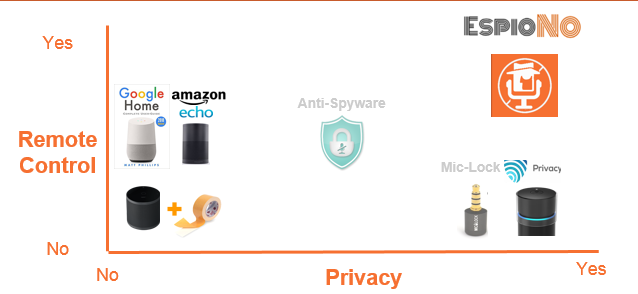
\includegraphics[width=\textwidth]{whatsoutthere.png}
\caption{What is out there}
\label{fig:What is out there}
\end{figure}

\end{itemize}



\subsection{Business planning}
\begin{itemize}
\item In the first stage, say 3 months, we will concentrating on developing the first minimal viable prototype. Which will be use to validate our technical solution and
demonstrate the viability to potential customer and invester. 
\item After we got enough feedback, and seed investment we will soon move into next stage, which will spend about 2 month, and finalize at least 20 prototypes 
which will be used to exhibits in conference and conduct in-field experiment to improve the user experience and 
collect pre-orders to prepare the mass production. 
\item After that we will settle down the first beta batch and contact manufacturers to massively produce our product.
The profits we earn at this stage is expected to be able to support ourself and start to feedback to our investers.
\item If everything goes well, it is time for us to plan for the long term. This kind of business is not sustainable just with such small device, especially when your 
business is depending on others product. We do have the suggestion from Yvo Desmedt that make a homomorphic encrypted smart speaker. This object is too big for us as 
a start-up, but it is very hopeful for a sustainable business. Which means we can expand our business to the whole LOT industry, to all the smart devices that might encounter
privacy problem. We can build our ecosystem and grow strong. With such expectation. we are going to seeking more investment to work on homomorphic remote computation used 
in speech recognition area.
\end{itemize}


\section{Business development process}
\label{sec:Business development process}
We have a detailed roadmap for how to spending money in chart \ref{chart:Financial detail 1} and \ref{chart:Financial detail 2}. 
\begin{table}[]
    \caption{Financial detail 1}
    \begin{tabular}{|l|l|l|l|l|l|l|l|l|l|l|}
        \hline
                                 & M1  & M2  & M3  & M4  & M5  & M6   & M7   & M8   & M9   & M10   \\ \hline 
    Volumes                      &     &     &     &     &     & 0    & 500  & 500  & 500  & 800   \\ \hline
    Unit price                   &     &     &     &     &     & 35   & 35   & 35   & 35   & 35    \\ \hline
    Revenues                     &     &     &     &     &     & 0.0  & 17.5 & 17.5 & 17.5 & 28.0  \\ \hline
                                 &     &     &     &     &     &      &      &      &      &      \\ \hline
    marketing                    &     &     &     &     &     &      &      &      &      &      \\ \hline
    Website (collect pre-orders) &     &     & -4  & -2  & -1  & -1   & -1   & -1   & -1   & -5   \\ \hline
    Communication campaigns      &     &     & -5  & -5  & -5  & -5   & -10  & -10  & -4   & -4   \\ \hline
    Events                       &     &     &     &     &     & -2   &      &      & -5   &      \\ \hline
    Advertising                  &     &     &     &     &     &      &      &      &      &      \\ \hline
    Human resource costs         &     &     &     &     &     &      &      &      &      &      \\ \hline
    Salary for developing MVP    & -5  & -5  & -5  &     &     &      &      &      &      &      \\ \hline
    Building 20 prototypes       &     &     &     & -10 & -10 &      &      &      &      &      \\ \hline
    Developing Beta batch        &     &     &     &     &     & -15  & -15  &      &      &      \\ \hline
    Long-term development cost   &     &     &     &     &     &      &      & -10  & -10  & -10  \\ \hline
                                 &     &     &     &     &     &      &      &      &      &      \\ \hline
    Fixed costs                  &     &     &     &     &     &      &      &      &      &      \\ \hline
    Equipment                    & -10 &     &     &     &     &      &      &      &      &      \\ \hline
    Models                       &     &     &     &     &     &      & -20  &      &      &      \\ \hline
    Material                     & -10 &     &     &     &     & 0    & -4   & -4   & -4   & -6.4 \\ \hline
    Storage and delivery         &     &     &     &     &     & 0    & -2.5 & -2.5 & -2.5 & -4   \\ \hline
    Cash                         & -25 & -5  & -14 & -17 & -16 & -23  & -35  & -10  & -9   & -1   \\ \hline
    Cumulate cash                & -25 & -30 & -44 & -61 & -77 & -100 & -135 & -145 & -154 & -155  \\ \hline
    \end{tabular}
    \label{chart:Financial detail 1}
\end{table}

\begin{table}[]
    \caption{Financial detail 2}
    \begin{tabular}{|l|l|l|l|l|l|l|l|l|l|}
        \hline
                                 & M11  & M12  & M13   & M14   & M15   & M16   & M17   & M18   & M19   \\ \hline
    Volumes                      & 1200 & 2000 & 2500  & 3000  & 3500  & 4000  & 5000  & 6000  & 7000  \\ \hline
    Unit price                   & 35   & 35   & 35    & 35    & 35    & 35    & 35    & 35    & 35    \\ \hline
    Revenues                     & 42.0 & 70.0 & 87.5  & 105.0 & 122.5 & 140.0 & 175.0 & 210.0 & 245.0 \\ \hline
                                 &      &      &       &       &       &       &       &       &       \\ \hline
    marketing                    &      &      &       &       &       &       &       &       &       \\ \hline
    Website (collect pre-orders) & -2   & -2   & -2    & -2    & -2    & -2    & -2    & -2    & -2    \\ \hline
    Communication campaigns      & -4   & -4   & -2    & -2    & -2    & -2    & -2    & -2    & -2    \\ \hline
    Events                       &      & -5   &       &       &       &       &       &       &       \\ \hline
    Advertising                  &      &      &       &       &       &       &       &       &       \\ \hline
    Human resource costs         &      &      &       &       &       &       &       &       &       \\ \hline
    Salary for developing MVP    &      &      &       &       &       &       &       &       &       \\ \hline
    Building 20 prototypes       &      &      &       &       &       &       &       &       &       \\ \hline
    Developing Beta batch        &      &      &       &       &       &       &       &       &       \\ \hline
    Long-term development cost   & -10  & -10  & -10   & -10   & -10   & -10   & -10   & -10   & -10   \\ \hline
                                 &      &      &       &       &       &       &       &       &       \\ \hline
    Fixed costs                  &      &      &       &       &       &       &       &       &       \\ \hline
    Equipment                    &      &      &       &       &       &       &       &       &       \\ \hline
    Models                       &      &      &       &       &       &       &       &       &       \\ \hline
    Material                     & -9.6 & -16  & -20   & -24   & -28   & -32   & -40   & -48   & -56   \\ \hline
    Storage and delivery         & -6   & -10  & -12.5 & -15   & -17.5 & -20   & -25   & -30   & -35   \\ \hline
    Cash                         & 10   & 23   & 41    & 52    & 63    & 74    & 96    & 118   & 140   \\ \hline
    Cumulate cash                & -145 & -122 & -81   & -29   & 34    & 108   & 204   & 322   & 462    \\  \hline
    \end{tabular}
    \label{chart:Financial detail 2}
\end{table}

From the tables we also generate a chart of cash flow \ref{fig:Cash flow}.

\begin{figure}[!htb]
    \centering
    \caption{Cash flow}
    \label{fig:Cash flow}
    \begin{tikzpicture}
        \begin{axis}[xlabel={Month },ylabel={Cash/K\$}]
    \addplot+[sharp plot]
    coordinates
    { (1,-25)
      (2,-30 )
      (3,-44)
      (4,-61)
      (5,-77)
      (6,-100)
      (7,-135)
      (8,-145)
      (9,-154)
      (10,-155)
      (11,-145)
      (12,-122)
      (13,-81)
      (14,-29)
      (15,34)
      (16,108)
      (17,204)
      (18,322)
      (19,462)
      };
\end{axis}
\end{tikzpicture}
\end{figure}
Clearly we woud need a lot of investment in the first stages. After mass production starts, we will be able to earn profits. And based on the assumption that we have
enough preorders and the subsequent sale goes pretty well. We will reach the balance point after month 14.

\section{Self evaluation}
\subsection{Course study}
To be honest, the subject of this summer school is my third choice. It is kind of hard for me to follw the lectures although I know they are just outlines of the subject
Cyber security and Privacy. However, I still feel learnd something. The guest lecture from Sergiu Carpov about CINGULATA, a toolchain for privacy preserving applications
is really inspiring for me. It use the homomorphic encryption technology to achieve computation on original data without knowing what they are. This idae is amazing to me and
we included it into the long term plan of our project.\\
Generally speaking, I was not really following the lecture but some part of it impress me a lot.
\subsection{Team work}
I was so lucky to be teammate with Maaike, Mauro and Xiaotong. Our team works well with each other, each of us is kind of specialist in certain area which help
us to efficiently divide work into different parts and the outcomes are excellent.\\
I was acting as an electronic and hardware specialist in our team for my experience working in start-up doing the same job. I evaluate the cost and viability of the solution and 
provide my own suggestion on calibrating it. I also try to present part of our slides in the first pitch and it goes better than before. That was a big step for me.

\begin{figure}[!htb]
    \centering
    \includegraphics[width=0.6\textwidth]{team.png}
    \caption{Our Team}
    \label{fig:Our Team}
\end{figure}
\begin{figure}[!htb]
    \centering
    \includegraphics[width=0.6\textwidth]{name.png}
    \caption{The sign of our project}
    \label{fig:Our Team}
\end{figure}

Finally thank you for all of you who organized this summer school. It was an amazing experience!

\clearpage
\bibliography{II2202-report}
%%\bibliographystyle{IEEEtran}
\bibliographystyle{myIEEEtran}
%\appendix



\end{document}
